\section{Evaluation}
% Here should be the experimental setup, and results

We ran the experiments on the instructional machines, with Intel(R) Core(TM) i5-4570 CPU @ 3.20GHz, with 8GB RAM.

\subsection{Clock Resolution}

We experimented on a single machine on the resolution of both \texttt{clock\_gettime} and \texttt{rdtscp}.

We used the real time clock for \texttt{clock\_gettime}, and obtained 1ns resolution, which agrees what we get with \texttt{clock\_getres}. For \texttt{rdtscp}, experiments give 1 cycle difference. To transform it into nanoseconds, we subsequently measured the TSC frequency, which is constant on the machine(nonstop\_tsc and constant\_tsc flag are on), by sleeping for a period of time(3 seconds in the test) and counting how many ticks have passed. It revealed that the TSC frequency roughly agreed with CPU base frequency, 3.2GHz. So we used \texttt{rdtscp} for subsequent measurements.

\subsection{System Calls}

We measured trivial syscalls \texttt{getpid} and \texttt{getuid}, \texttt{getpid} took 366.6ns, and \texttt{getuid} took 364.7ns.

\subsection{Latency and Throughput}

We measured IPC performance on a single machine, and between two machines in the same LAN.

The latencies of all IPCs are stable at first, and grow up after a threshold, which means the bottleneck are changed during the process -- when packets are small a fixed time cost in the same order as system calls is dominant, but as they become larger, the transmission cost starts to take dominance.

On the other side, the throughput becomes larger as the packet size increases, but usually stops increasing at some point.

The measurement with pipe shows something interesting: the bandwidth first increases with the packet size, but after reaching around 16KiB packet size, the performance starts to deteriorate as the packet size grows up. We hypothesized the default 64KiB pipe buffer in Linux is the reason, but due to the limitation of the instructional machine, we cannot modify the pipe buffer size to verify such hypothesis.

\begin{figure}[!ht]
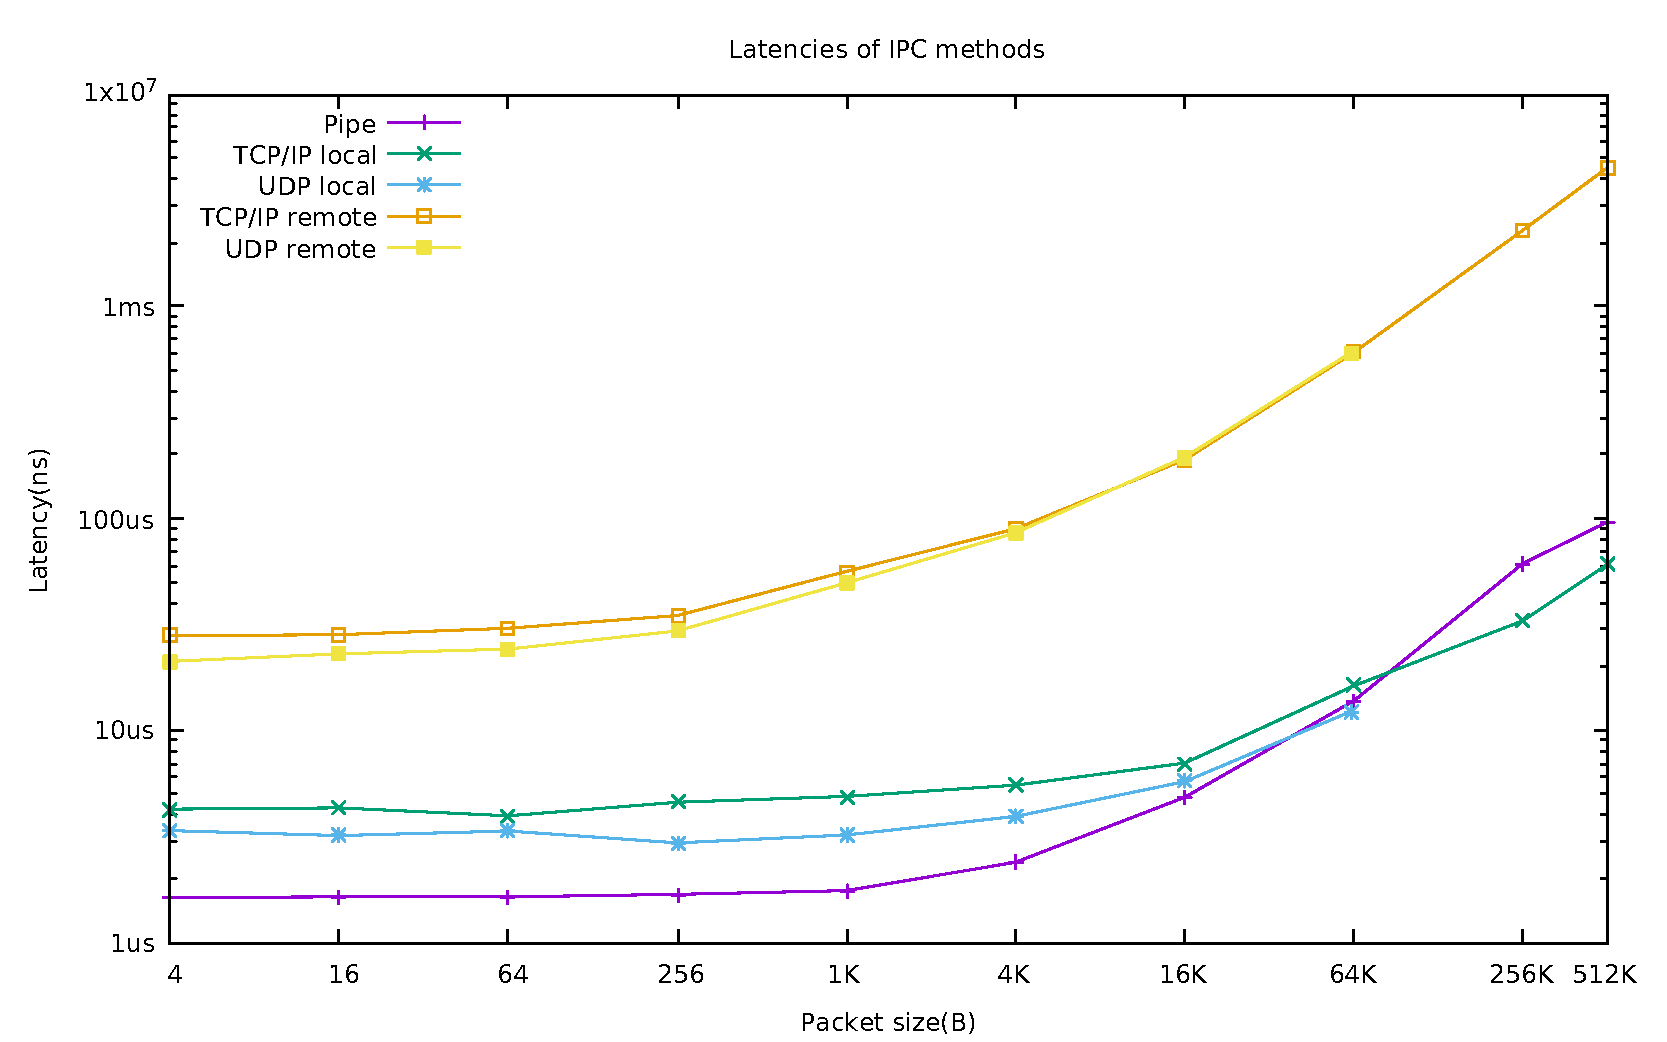
\includegraphics[width=.7\linewidth]{figures/latency}
\label{figure:latency}
\end{figure}

\begin{figure}[!ht]
    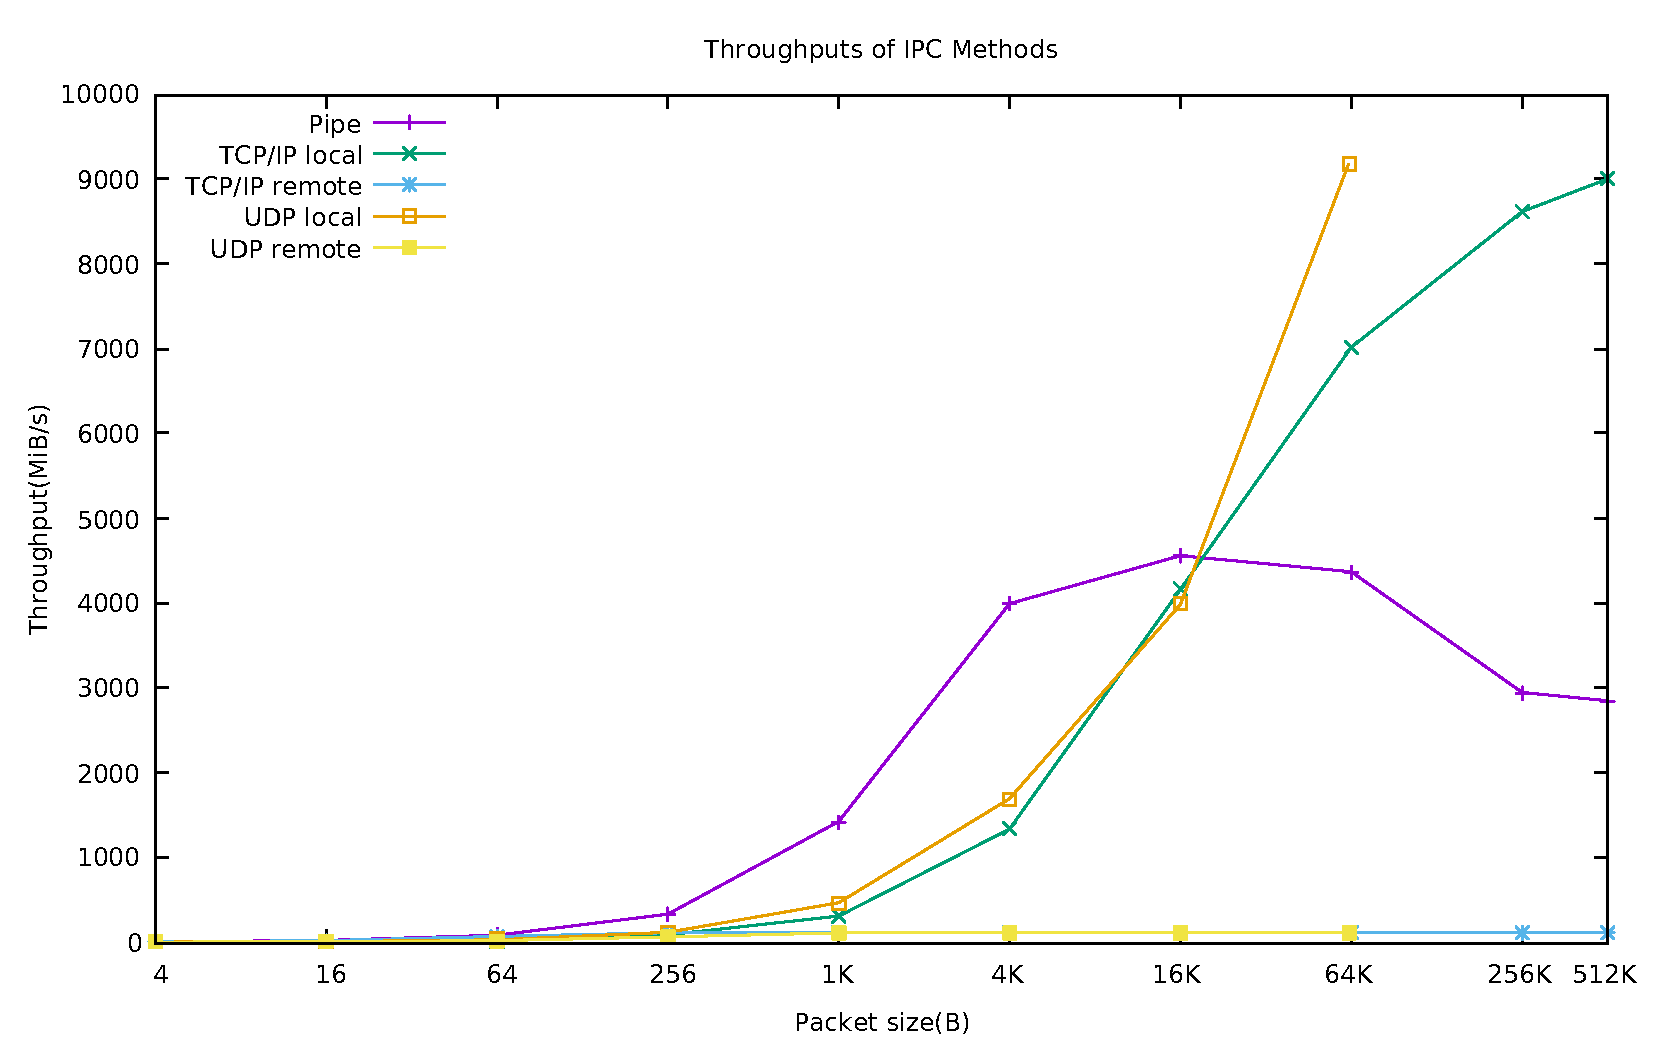
\includegraphics[width=.7\linewidth]{figures/throughput.pdf}
    \label{figure:throughput}
\end{figure}
